\begin{frame}[allowframebreaks]{PixelRNN – Pixel Recurrent Neural Network}
    \textbf{Introduced by:} van den Oord et al. (2016)

    \vspace{1em}
    \textbf{What is PixelRNN?}

    \begin{itemize}
        \item PixelRNN is a generative model specifically designed for image generation.
        \item It models the joint distribution of all pixels in an image by predicting one pixel at a time.
        \item Pixels are generated in a raster-scan order (left to right, top to bottom).
        \item Uses an autoregressive approach, where each pixel is generated conditioned on all previously generated pixels.
    \end{itemize}  

    \framebreak
    
    \textbf{Core Idea:}
    The model factorizes the image distribution as:
    \[
    p(\mathbf{x}) = \prod_{i=1}^{n} p(x_i \mid x_1, x_2, \ldots, x_{i-1})
    \]
    where each pixel $x_i$ is conditioned on all previous pixels $(x_1, x_2, \ldots, x_{i-1})$.

    Each pixel's value (such as its RGB channels) is predicted based on all preceding pixels using a recurrent neural network, allowing the model to capture complex dependencies and structures within the image.
    
    \framebreak
    \textbf{Architecture of PixelRNN}

    \begin{enumerate}
        \setlength{\itemsep}{-0.25em}
        \item \textbf{Input Representation:}
        \begin{itemize}
            \setlength{\itemsep}{-0.25em}
            \item Each image is a 2D grid of pixels.
            \item Each pixel can have multiple channels (e.g., RGB).
        \end{itemize}

        \item \textbf{Autoregressive Modeling:}
        \begin{itemize}
            \item For each pixel, the model learns $p(x_{i,j} \mid x_{<i,j})$, where $x_{<i,j}$ are all pixels above and to the left of the current pixel $(i, j)$.
        \end{itemize}

        \item \textbf{RNN Layers:}
        \begin{itemize}
            \item Uses RNNs along the rows of the image:
            \begin{itemize}
                \item \textbf{Row LSTM:} Processes one row at a time from left to right.
                \item \textbf{Diagonal BiLSTM:} Processes diagonals in the image to improve context.
            \end{itemize}
        \end{itemize}

        \item \textbf{Masked Convolutions:}
        \begin{itemize}
            \item Prevent the model from “seeing the future” pixels.
            \item Each convolution is masked to preserve the autoregressive property.
        \end{itemize}
    \end{enumerate}

    \framebreak
    \begin{figure}
        \centering
        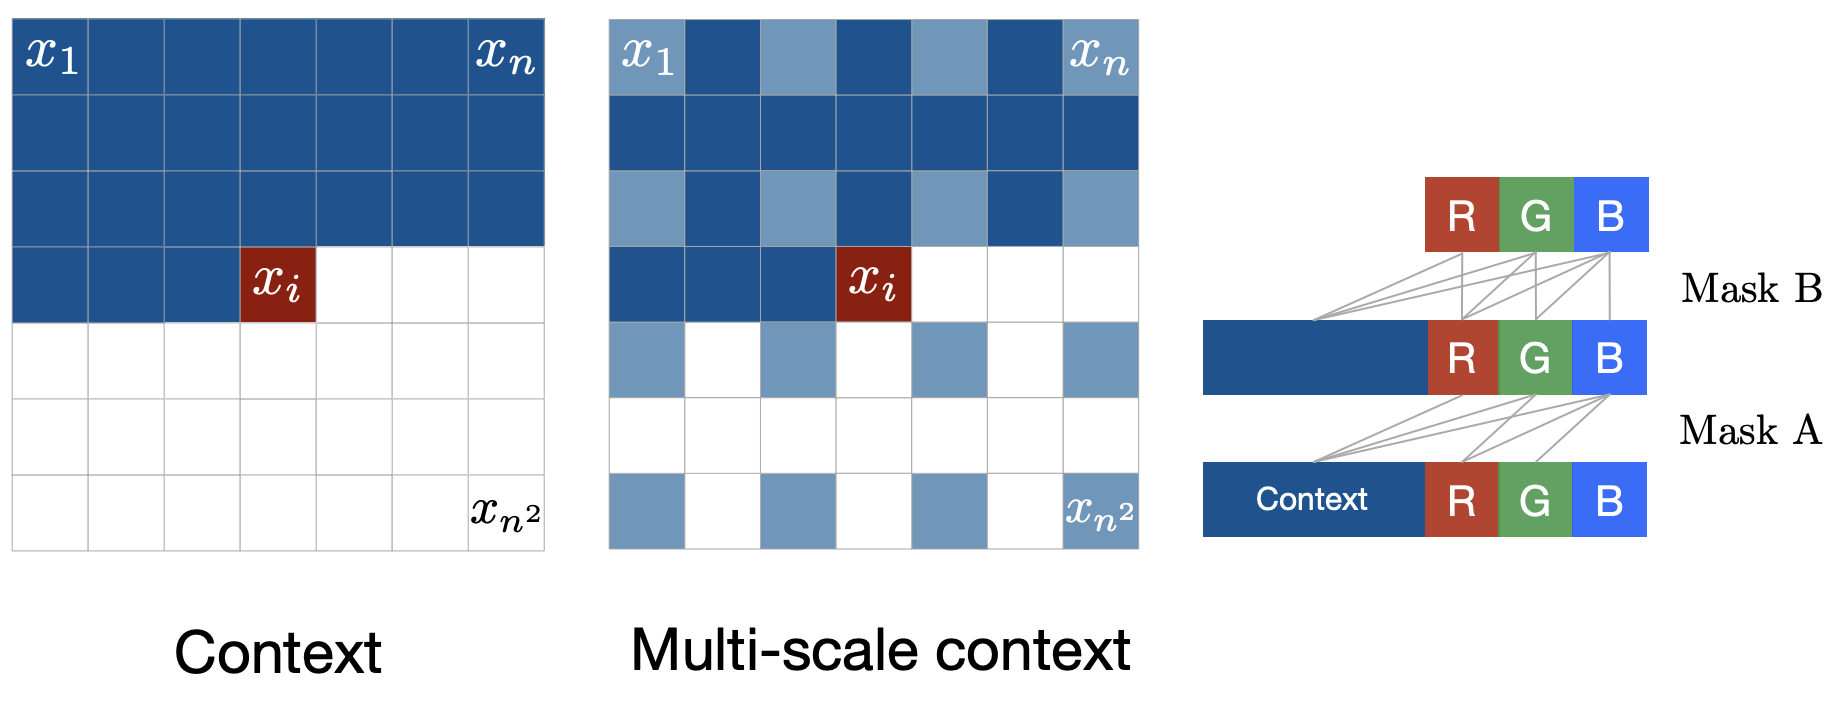
\includegraphics[height=1.0in]{images/autoregressive/pixel-rnn.png}
        \caption*{Left: To generate pixel xi one conditions on all the previously generated pixels left and above of xi. Center: To generate a pixel in the multi-scale case we can also condition on the
subsampled image pixels (in light blue). Right: Diagram of the
connectivity inside a masked convolution. In the first layer, each
of the RGB channels is connected to previous channels and to the
context, but is not connected to itself. In subsequent layers, the
channels are also connected to themselves.}
    \end{figure}

    \framebreak

    \begin{columns}
        \begin{column}{0.4\textwidth}
            \textbf{Types of RNNs in PixelRNN}

            \begin{itemize}
                \item \textbf{Row LSTM:}
                \begin{itemize}
                    \item Applies a 1D LSTM across each row.
                    \item Information flows left-to-right in each row.
                    \item Maintains the autoregressive structure.
                \end{itemize}

                \item \textbf{Diagonal BiLSTM:}
                \begin{itemize}
                    \item Applies a 2D LSTM diagonally across the image.
                    \item Allows pixels to be conditioned on a broader context.
                \end{itemize}
            \end{itemize}
        \end{column}
        \begin{column}{0.6\textwidth}
            \begin{figure}
                \centering
                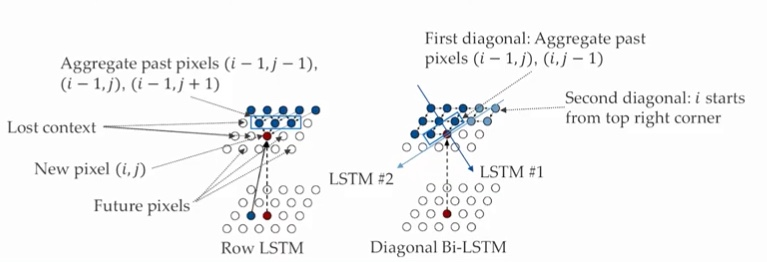
\includegraphics[width=1.1\textwidth,keepaspectratio]{images/autoregressive/pixel-rnn-networks.png}
                \caption*{PixelRNN architecture with Row LSTM and Diagonal BiLSTM. The model processes pixels in a raster-scan order, ensuring that each pixel is conditioned on all previously generated pixels.}
            \end{figure}
        \end{column}
    \end{columns}

    \framebreak
    \textbf{Training and Inference:}
    \begin{itemize}
        \item \textbf{Training:} The model is trained using maximum likelihood estimation (MLE) to maximize the joint probability of the pixels in the training images.
        \item \textbf{Inference:} During inference, pixels are generated sequentially, starting from a blank canvas and conditioning each new pixel on all previously generated pixels.
        \item \textbf{Sampling:} The model can sample new images by repeatedly predicting the next pixel based on the current image context.
    \end{itemize}

    \begin{figure}
        \centering
        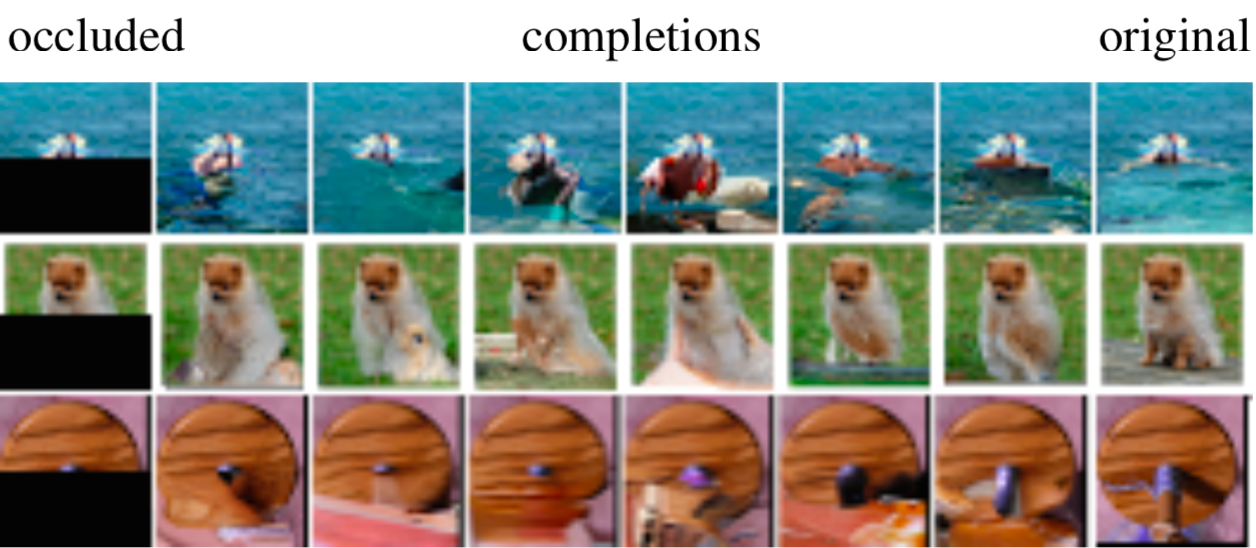
\includegraphics[width=\textwidth,keepaspectratio]{images/autoregressive/example-pixel-rnn.png}
        \caption*{Image completions sampled from a PixelRNN.}
    \end{figure}

    \framebreak
    \textbf{Pros:}
    \begin{itemize}
        \item Capable of generating high-quality images with complex structures.
        \item Effective at capturing long-range dependencies in images.
    \end{itemize}

    \textbf{Cons:}
    \begin{itemize}
        \item Computationally intensive due to sequential processing of pixels.
        \item Slower inference compared to parallelizable models like PixelCNN.
    \end{itemize}
\end{frame}